\documentclass{article}

\usepackage[utf8]{inputenc}
\usepackage[T1]{fontenc}
\usepackage{microtype}

\usepackage{newspaper}

\date{17-nov-1931}
%\date{\today}
\currentvolume{1}
\currentissue{1}

%% [LianTze] The newspaper package also provides 
%% these commands to set various metadata:

%% The banner headline on the first page
%%   (The colon after s: is to get a more
%%   modern majuscule s in this font instead of 
%%   the medieval tall s. For anyone interested 
%%   in the history: 
%%  http://medievalwriting.50megs.com/scripts/letters/historys.htm)
\SetPaperName{Monatshefte}

%% The name used in the running header after
%% the first page
%\SetHeaderName{Monatshefte für Mathematik}
\SetHeaderName{Monatshefte}

%% and also...
\SetPaperLocation{Königsberg GER}
\SetPaperSlogan{``Monatshefte für Mathematik: O seu canal de divulgação matemática.''}
\SetPaperPrice{n+1 Reais}


% [LianTze] times (the package not the font) is rather outdated now; use newtx (see later)
% \usepackage{times}
\usepackage{graphicx}
\usepackage{multicol}

\usepackage{picinpar}
%uasage of picinpar:
%\begin{window}[1,l,\includegraphics{},caption]xxxxx\end{window}


%% [LianTze] Contains some modifications
\usepackage{newspaper-mod}
%%... so now you can redefine the headline and byline style if you want to.
%% These can be issued just before any
%% byline or headline in the paper, to
%% individually style each article
%%
% \renewcommand{\headlinestyle}{\itshape\Large\lsstyle}
% \renewcommand{\bylinestyle}{\bfseries\Large\raggedright}


%%%%%%%%%  Front matter   %%%%%%%%%%

\usepackage{lipsum}

\begin{document}
\maketitle

\begin{multicols}{3}

    \byline{Primeiro teorema da incompletude}{Artur Avila}

    Teorema 1: \emph{"Qualquer teoria axiomática recursivamente enumerável e capaz de expressar algumas verdades básicas de aritmética não pode ser, ao mesmo tempo, completa e consistente. Ou seja, em uma teoria consistente, sempre há proposições que não podem ser demonstradas nem verdadeiras, nem falsas."}. Teorema 2: \emph{"Uma teoria, recursivamente enumerável e capaz de expressar verdades básicas da aritmética e alguns enunciados da teoria da prova, pode provar sua própria consistência se, e somente se, for inconsistente."}
    \begin{window}[2,r,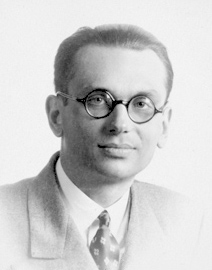
\includegraphics[width=1.0in]{images/kurt.jpg},\centerline{Kurt Gödel}]  
        A surpreendente prova de Gödel mostrou que a suposição de \emph{Hilbert}, de que toda a matemática é completa, consistente e pode ser demonstrada a partir de um conjunto finito de axiomas estava errada.
    \end{window}
    %First Incompleteness Theorem: "Any consistent formal system F within which a certain amount of elementary arithmetic can be carried out is incomplete; i.e., there are statements of the language of F which can neither be proved nor disproved in F." (Raatikainen 2015)

%\begin{window}[2,r,\includegraphics[width=1.0in]{atom.jpg},\centerline{The Atom}] The \verb+multicol+ package allows using multiple columns without starting a new page.  Using floats is not possible in a columns environment, however with the \verb+picinpar+ package, I can set a picture inside a block of text---just like you one you see here.  Isn't \LaTeX{} cool?
%And now we're just filling more space, and yet more space.  
%\end{window}
    \closearticle

    %\byline{O Paradoxo de Russel}{Richard Stallman}
    \headline{O Paradoxo de Russel}
    \begin{window}[2,r,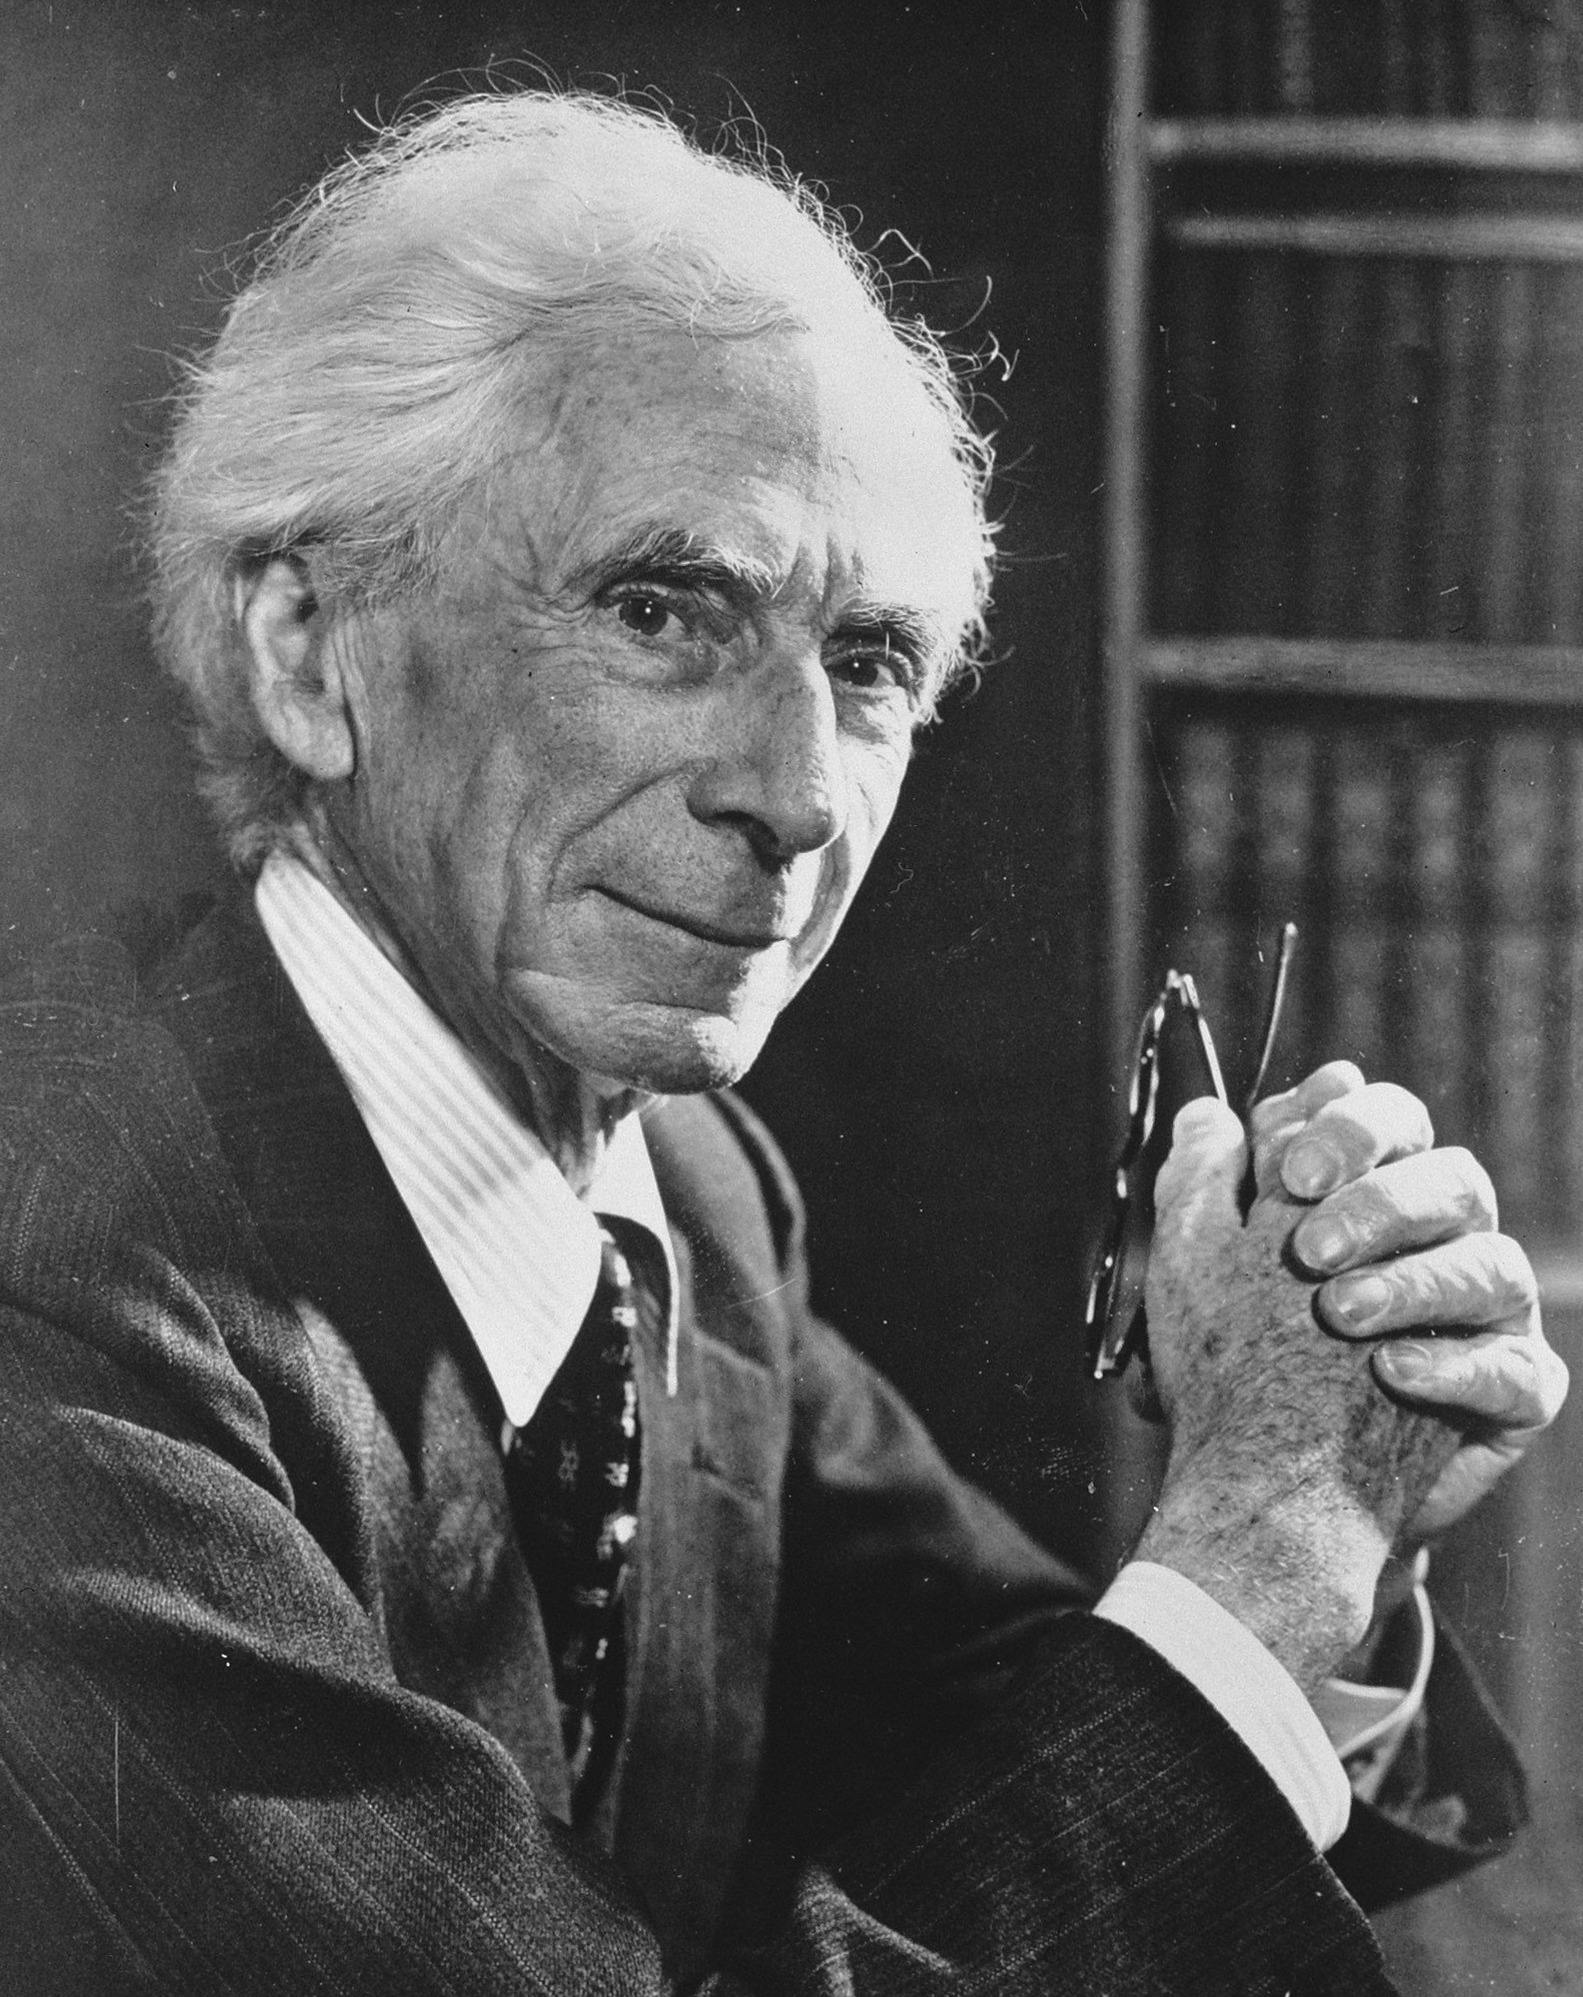
\includegraphics[width=1.0in]{images/russel.jpg},\centerline{Bertrand Russel}]  
    O conhecido paradoxo é posto da seguinte maneira: \emph{Consideremos o conjunto de todos os conjuntos que não tem a si próprio como elemento, ou seja, $D = \{X | X \not\in X\}$}. O paradoxo pode ser obtido quando questionado: $D$ percente a $D$? Se supormos que $D$ pertence a $D$ e observarmos a regra de definição do conjunto, temos $D \not\in D$. Por outro lado, se inicialmente supormos que $D$ não pertence a $D$, ele satisfaz a regra de definição do conjunto e consequentemente $D \in D$, o que contradiz nossa suposição. O paradoxo do barbeiro, é uma maneira ilustrativa daquele paradoxo. Suponhamos que em uma cidade exista \emph{apenas um} barbeiro. Nesta cidade cada homem mantém-se bem barbeado e para isso utiliza-se de exclusivamente um, de dois métodos: $1º)$ Ele vai ao barbeiro. $2º)$ Ele corta sua própria barba. Nesse caso, quem barbeia o barbeiro?
    \end{window}
    \closearticle

    \byline{Programa de Hilbert}{Adonai Sant'anna}
    \begin{window}[2,r,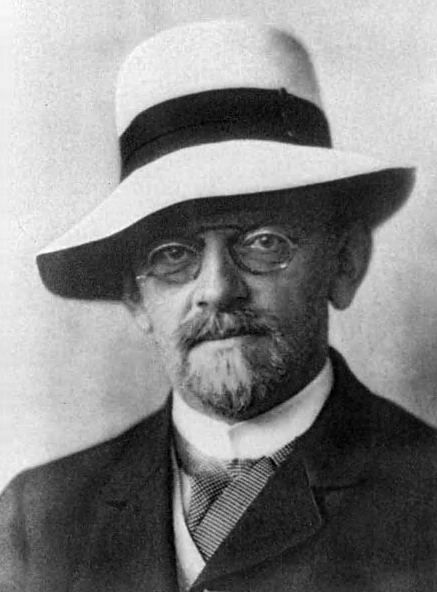
\includegraphics[width=1.0in]{images/hilbert.jpg},\centerline{David Hilbert}] 
        No início do século XX houveram tentativas de clarificar os fundamentos da matemática, nelas foram encontrados paradoxos e inconsistências. Hilbert então propõe uma solução: encontrar um conjunto finito de axiomas que sejam completos e consistentes, isto é por completo, qualquer sentença no sistema em questão ou é provável, ou sua negação é provável. Por consistente, um teorema e sua negação não podem ser provadas, isto é, utilizando-se dos axiomas e das regras de inferência, não é possível demonstrar $P$ e $\lnot P$. Alguns pontos que essa fundamentação deveria possuir são: $\cdot$ formalização de \emph{toda} a matemática; $\cdot$ Completeza (sintética); $\cdot$ Consistência; $\cdot$ Conservação;  $\cdot$ Decidibilidade;
    \end{window}
    Gödel mostra que é impossível formalizar toda a matemática, e isto sem recorrer ao que se chama 'Argumento do regresso' ou 'regressão ao infinito'. Mostra também que um sistema aritmético semelhante ao de Peano não pode demonstrar sua própria consistência. E que não há algoritmo para decidir se uma dada sentença é um teorema (isto é, é passível de ser provado/demonstrado).
    Não obstante, a matemática 'comum' pode ser formalizada de forma satisfatória, um exemplo é a Teoria de Conjuntos de Zermelo e Fraenkel (ZFC)com a lógica de primeira ordem, que são geralmente aceitas.
    Embora sistemas como o de Peano sejam incompletos, existem outros sistemas que são completos. Exemplos são o \emph{teorema da completeza de Gödel} e em teoria algébrica de corpos fechados, dados alguns requisitos.
    Tarski descobriu que a teoria dos corpos Reais fechados é decidível, isto é, qualquer sentença nesse contexto ou é passível de demonstração ou sua negação o é.
    Com o \emph{axioma Cantor-Dedekind} esse algoritmo consegue decidir se uma dada sentença na geometria euclidiana, é verdadeira ou não.
    \closearticle
    
    \newpage
    \byline{Biografia}{Newton da Costa}
Kurt Friedrich Gödel nasceu no dia 28 de Abril de 1906 em Brünn, Moravia, agora República Checa, numa família germânica proprietária de uma indústria de têxteis. Adquiriu a nacionalidade Checa, logo após a queda do império Austro-Húngaro, no final da Primeira Guerra Mundial. Mais tarde viria a adquirir a nacionalidade Austríaca e, por anexação da Áustria à Alemanha durante o período Nazi, conseguiu a nacionalidade Germânica. Após o final da Segunda Guerra Mundial tornou-se cidadão americano.
Em pequeno demonstrava já um enorme interesse e curiosidade pela compreensão das coisas. Frequentou a escola alemã no ensino primário e secundário e completou o seu primeiro percurso escolar com distinção. Tinha um especial interesse por História e Matemática.

Em 1920, quando o seu irmão foi estudar medicina para Viena, começou a interessar-se mais por matemática. Aos 18 anos conseguiu juntar-se ao seu irmão na Universidade de Viena. Nessa altura já dominava bastantes tópicos matemáticos de nível universitário. Embora inicialmente estivesse interessado em física teórica, frequentou também aulas de matemática e de filosofia. 

Começou por dedicar-se ao estudo de Teoria dos Números, mas ao participar numa série de seminários de lógica matemática, interessou-se pelo assunto.
A frequência de um curso sobre completude e consistência de teorias matemáticas, dirigido por David Hilbert em Bolonha, marcou o seu futuro enquanto matemático. Em 1928, Hilbert publicou um livro sobre lógica matemática onde levantou um problema que viria a ser o assunto da tese doutoral de Gödel:

“Será que os axiomas de um sistema formal são suficientes para demonstrar todas as verdades consistentes com esse sistema?”

Aos 23 anos completou a sua tese sob a supervisão de Hans Hahn. Nela estabeleceu o seu teorema da completude. Em 1931 publicou aquele que é hoje conhecido como o seu teorema da incompletude, onde demonstrou que um sistema formal consistente não pode ser completo e que a consistência dos axiomas não pode ser provada pelo sistema formal. Estes teoremas acabaram de vez com a procura de um conjunto finito de axiomas suficientes para toda a matemática e mostram que nem todas as questões matemáticas são passíveis de ser respondidas.
Em 1932, Gödel tornou-se professor na Universidade de Viena. Como resultado da ascensão de Hitler ao poder na Alemanha e do clima instável que se vivia na Áustria, acabou por sofrer uma depressão em consequência da morte de um dos seus amigos.

Em 1933 viajou pela primeira vez aos Estados Unidos onde conheceu Albert Einstein, de quem se tornou amigo. Visitou, em Princeton, o Instituto de Estudos Avançados onde dirigiu uma série de seminários sobre os seus teoremas. 

Durante essa década deslocou-se várias vezes aos Estados Unidos para apresentar seminários.

Em 1938 casou-se com Adele Nimbursky, uma bailarina divorciada que conhecia há dez anos. Não tiveram filhos.
Nesse ano, a anexação da Áustria à Alemanha trouxe mudanças na organização da Universidade de Viena. O seu cargo de professor auxiliar foi extinto e viu-se obrigado a procurar outra posição. Com o início da II Grande Guerra, em 1939, corria o risco de ser chamado a combater pelo exército Nazi. Decidiu assim abandonar a Europa.

Tendo como objetivo chegar aos Estados Unidos, viu-se obrigado a viajar através da Ásia, passando pelo Japão. Chegou a São Francisco em 1940. Percorreu toda a América até Princeton onde conseguiu uma posição, no Instituto de Estudos Avançados.

Ainda nesse ano publicou um trabalho sobre a “consistência do Axioma da Escolha e da generalização da hipótese do continuum”, com os axiomas da teoria dos conjuntos, hoje um clássico da matemática moderna. Também nesse ano demonstrou a existência de soluções paradoxais das equações de Einstein para a relatividade geral. 

Em 1946 tornou-se membro permanente do Instituto de Estudos Avançados. Os seus interesses regressaram então à física teórica e à filosofia. 

Em 1974 foi-lhe atribuída a “National Medal of Science”.


    \begin{window}[2,r,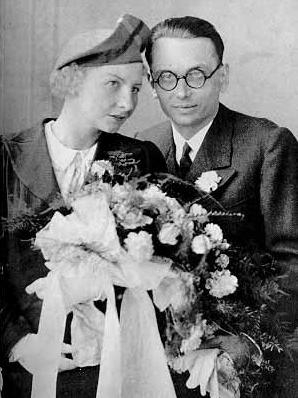
\includegraphics[width=1.0in]{images/esposa.jpg},\centerline{Gödel e Adele}]  
Os últimos anos da sua vida foram marcados por períodos de instabilidade mental. Vivia obcecado pela possibilidade de alguém o envenenar. Todas as suas refeições tinham de ser primeiro provadas. Em 1977 a sua mulher, que testava todas as suas refeições, foi hospitalizada e Gödel deixou de comer.
Morreu de má nutrição em 14 de Janeiro de 1978.
    \end{window}
\closearticle

\headline{A 'revolução' de Gödel}
Há mais verdades do que podemos provar.
Por sorte, houve várias tentativas de explicar de forma didática os teoremas da incompletude, para que todos pudessem compreender o grande feito do "senhor por quê".
Em resumo, o que Gödel fez foi usar a matemática para provar que a matemática não consegue ser sempre comprovada por meio de cálculos. 
Em qualquer sistema há afirmações que são verdadeiras, mas que não podem ser comprovadas.
\closearticle
\headline{Mudança de paradigma}
Os teoremas da incompletude revolucionaram a matemática e inspiraram pessoas como John von Newman, um dos criadores da Teoria dos Jogos, e Alan Turing, criador do sistema matemático que viabilizou os computadores que usamos hoje.
Também se mostraram valiosos para a Tecnologia da Informação. 
O reconhecimento de que existem coisas que não podem ser provadas estabeleceu um limite ao que os computadores são capazes de resolver, evitando a perda de tempo de tentar alcançar o que é impossível.
Muitos apostam que os teoremas de Gödel impactarão outros campos. O físico, matemático e filósofo Roger Penrose, por exemplo, considera que eles poderão ajudar a descobrir uma nova física que explique os mistérios da consciência.
\closearticle


\headline{Temores e angústias}
    \begin{window}[2,r,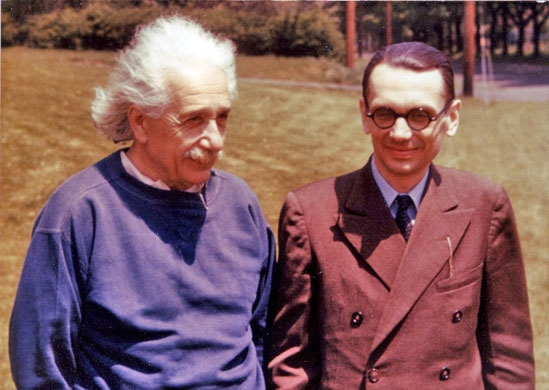
\includegraphics[width=1.0in]{images/Albert.jpg},\centerline{Gödel e Einstein}]  
Ao final da carreira, quando estava prestes a se aposentar, Einstein comentou que continuava a ir a seu escritório apenas para ter o privilégio de caminhar com Gödel, algo que fez até pouco antes de morrer, em 1955.
Os dois cientistas batiam papo durante o trajeto até o Instituto de Estudos Avançados de Princeton. Alguns pensamentos de Gödel, porém, eram obscuros. Sempre viveu atormentado por temores e angústias. Tinha, por exemplo, pavor de ser envenenado.
    \end{window}
\closearticle
\headline{Terminologia}
Dado um sistema formal, temos abaixo algumas definições:


Completeza/completude: neste texto refere-se à completeza sintética, que dado um sistema formal $F$ e uma sentença $S$ ocorre de $S$ ser um teorema, ou $\lnot S$ ser um teorema, podendo, no caso de inconsistência serem ambos teoremas.

Alfabeto: conjunto finito de símbolos. Exemplo: \{a,b,3, 4, 5, +, =\}.

Fórmulas: quaisquer sequências de símbolos do alfabeto dado. Exemplo: \{ab=+, ++++, ab, abb, aabb\}

Fórmulas bem formadas/fbf's: fórmulas que expressam algum significado. Exemplo: \{a=b, a+b, a+a+a=b=4a\}, não são fbf's \{a=, ab+=, a=+\}.

Axioma: um conjunto de fórmulas bem formadas.

Demonstração/prova: É uma sequência $B_1, B_2, ..., B_n$ de fbf's cujo cada termo é um axioma ou uma consequência direta de pelo menos alguma das fórmulas que antecedem ela nesta sequência pelo uso de alguma regra de inferência.

Teorema: A última fórmula de uma demonstração.

Inconsistência: Quando é possível provar uma sentença e sua negação, por exemplo: $A$ e $\lnot A$.

Decidibilidade: Quando existe um algoritmo capaz de identificar se uma dada fbf do sistema é ou não um teorema.

Provável: Nesse contexto exceto mencionado contrário, é o que pode ser provado.

Paradoxo: Sentença aparentemente verdadeira que quando analisada observa-se ser contraditória.

\headline{Referências}

https://www.bbc.com/portuguese/geral-43618903

http://evo2.org/o-teorema-da-incompletude-de-godel-a-descoberta-matematica-n%C2%BA-1-do-seculo-xx/

http://evo2.org/o-teorema-da-incompletude-de-godel-a-descoberta-matematica-n%C2%BA-1-do-seculo-xx/

http://e-escola.tecnico.ulisboa.pt/personalidade/godel-kurt-friedrich

O que é um axioma. Sant'Anna, A. S. Barueri, SP: Manole, 2003.
\closearticle

\end{multicols}
%\newpage
%\begin{multicols}{3}
%    \byline{Programa de Hilbert}{Alfaiate}
%\en:w

\end{document}
